\chapter{系统分析}
	
	串口作为计算机的一种标准接口,其硬件实现简单,且数据和控制信息是一位接一位的串行地传输下去的,比较适合于远距离传输,传输线路少。但是近年来由于其传输速度慢,扩展不方便,不支持热插拔等缺点,导致其逐渐的被各种设备所抛弃。而USB接口由于其速度快、连接灵活、支持即插即用等特点成为了设备标配接口。但是串口由于其在计算机与设备的通信中有USB无法企及的优点。
	
	本次设计的工作包括一个USB口转串口的驱动部分、基于USB口转串口驱动的应用层接口部分、windows下的调试信息分析界面部分。其中的重点在于本论文将要描述的基于VxWorks的调试通道部分,包括驱动部分和应用层的接口部分。
	
	要编写VxWorks下的驱动程序必须先对VxWorks系统有一定的了解。下面我们先介绍一下VxWorks下完成我们的驱动程序所必需的关于VxWorks的知识,USB开发相关的技术和串口开发相关的技术 。

\section{VxWorks开发}
	VxWorks的基本构成部件由5个部分组成:板级支持包、wind内核、网络系统、文件子系统、IO系统。其结构如\autoref{fig:VxWorks系统结构}所示。
\begin{figure}[!h]
\centering
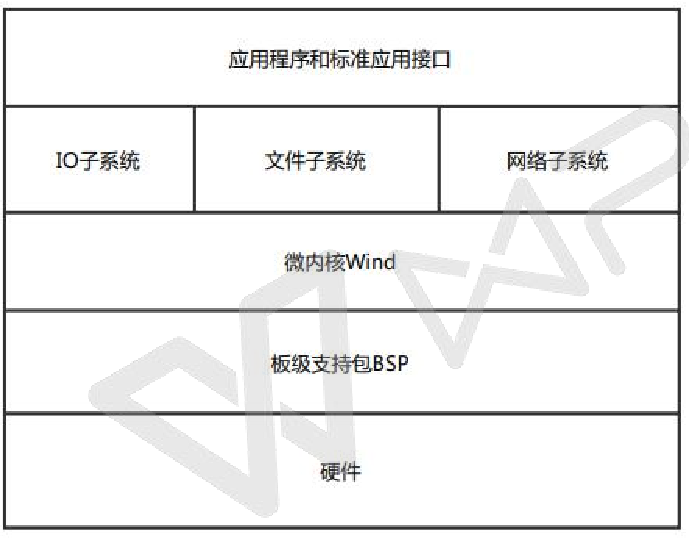
\includegraphics[width=.7\textwidth]{./graphics/VxWorks-sys-structure.pdf}
\caption{VxWorks系统结构}\label{fig:VxWorks系统结构}
\end{figure}

在本次的设计当中会使用到的部分包括VxWorks的wind内核部分和IO子系统部分,因此有必要介绍这两部分的相关内容。
	
\subsection{微内核wind}
	VxWorks采用微内核设计,其微内核被称为wind,支持多种硬件环境,包括X86、PowerPC、ARM等众多主流的处理器,同时还支持RISC、DSP技术,且在各种CPU平台上提供了统一的编程接口和一致的运行环境。微内核的设计保证了内核的高效、精简,由用户进程来实现大多数操作系统的功能,这使得系统具有模块化、结构清晰、可移植性强和可裁剪性好的特点。在微内核操作系统当中,设备驱动程序通常作为核外可裁剪的部分存在。对于操作系统内核来说,核外驱动就相当于一个普通的应用程序,因此对于系统内核的影响很小,编写和调试都很方便,同时可以避免数据流在不同级间的拷贝。
		
	内核作为操作系统的核心,负责控制这计算机上的所有硬件和软件资源,在必要的时候给应用程序分配硬件资源,并执行相应的操作命令。wind内核的主要功能如下:
\begin{itemize}
\item 系统内存管理

\item 任务调度

\item 任务间同步和通信

\item IO管理

\item 文件和网络系统管理
\end{itemize}

	Wind的主要特点在于高效的任务管理(提供无限数量的的多任务,具有256个优先级,灵活快速的调度机制)、方便的任务间通信(提供多种信号量,网络通信以及共享内存等)、高度可裁剪(内核最小可以裁剪到8K)。由于VxWorks操作系统模块化非常好,模块间的耦合度非常低,每个模块对外提供都是单独的头文件,比如任务调度,其头文件为taskLib.h,任务通讯如果用的队列,那其头文件就是msgQLib.h,如果是定时器管理,那其头文件就是timerLib.h,因此也让程序移植提供了很大的便利性。

\subsection{wind的任务调度}
	VxWorks下的任务即通用操作系统下所述的进程,是内核的基本运行单位,wind提供多任务环境,允许实时应用程序以一套独立任务的方式构筑(即程序可以由单个或多个任务来构成,每个任务是程序的一个实例),每一个任务拥有独立的执行线程和一套自己的系统资源,同时由于在VxWorks中对内存进行统一编址,在任务间进行资源共享也十分方便,而任务间的通信机制可以使得得这些任务的行为同步、协调。每一个开启的任务都有一个任务控制的数据结构来记录当前的任务的状态,供内核管理调度,这个控制块简记为TCB。控制块里包含了当前的状态、优先级、要等待的事件或资源、任务程序码的起始地址、初始堆栈指针等任务的上下文。
		
	操作系统的进程调度时机基本上都会选择在同一个地方:从内核状态退出之时,VxWorks也一样。从内核状态退出的时机主要有两个渠道:系统调用和中断。VxWorks与于通用操作系统的区别的关键点在于其必须能够迅速的响应外部中断,所以实时操作系统只是在响应速度上更快,而在响应时机上与通用操作系统并无区别。Vxworks区别于通用操作系统的另一个显著的特点是其划分运行级别,应用层程序可以直接调用内核函数,而不需要通过软中断的方式从应用层进入到内核层。VxWorks将任务被分为256个优先级,0最高,255最低;任务在被创建时就会被指定一个优先级,在运行时也可以通过taskPrioritySet()函数重新设定优先级。该函数的原型如下:
\lstset{language=C}
\begin{lstlisting}
STATUS taskPrioritySet
(
  int tid, /* task ID */
  int newPriority /* new priority */
) 
\end{lstlisting}
	
	在VxWorks中任务调度是基于优先级的,而且是可抢占式的调度方式,这样才能够区分实际情况下的不同状态的处理级别,对高优先级的情况进行优先响应。	VxWorks下对于应用层任务,推荐使用100-250之间的优先级,驱动层任务可以使用51-99之间的优先级。
	VxWorks中任务的状态通常有四种,这四种状态可以通过相应的函数控制其相互转化:
\begin{itemize}
\item \textbf{就绪态:}任务正在等待CPU资源,该状态下以优先级为序排列任务。
\item \textbf{休眠态:}任务正在等待除CPU资源之外的其他资源,当竞争使用某个资源,而资源当前不可得,就进入这个状态。
\item \textbf{延迟态:}任务正在等待一定时间的延时。当调用taskDelay 函数让任务延迟一段固定的时间时,任务所处的状态,此时任务无资格竞争使用CPU。
\item \textbf{悬置态:}任务无法执行,主要是用于调试一种状态,这种状态仅影响任务的执行而不影响任务的转换。
\end{itemize}

\begin{figure}[!h]
\centering
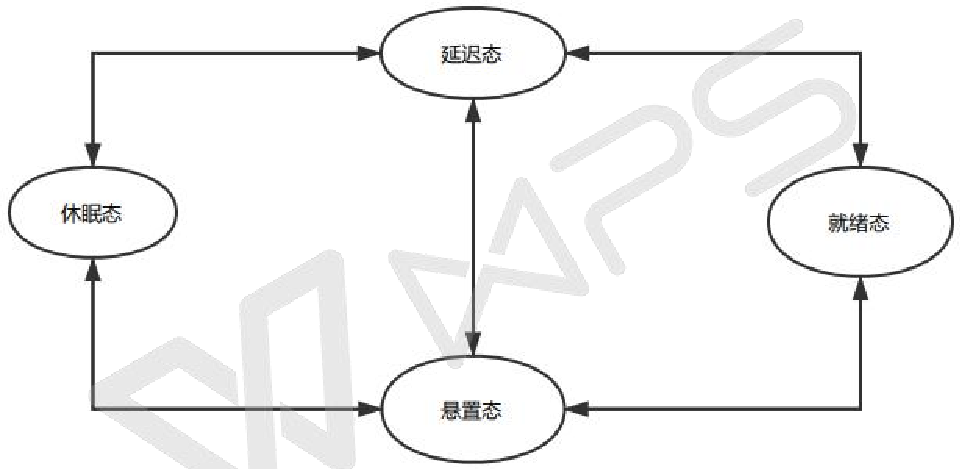
\includegraphics[width=.9\textwidth]{./graphics/vxworks-task-shift-diagram.pdf}
\caption{任务状态转换图}\label{fig:VxWorks状态转换图}
\end{figure}

	如\autoref{fig:wind任务调度}的wind内核任务调度框图展示了内核中构建了四种状态队列,通过TCB中任务状态的变化,由内核对其进行调度,并把就绪的任务加入到就绪队列等候CPU资源。
\begin{figure}[!h]
\centering
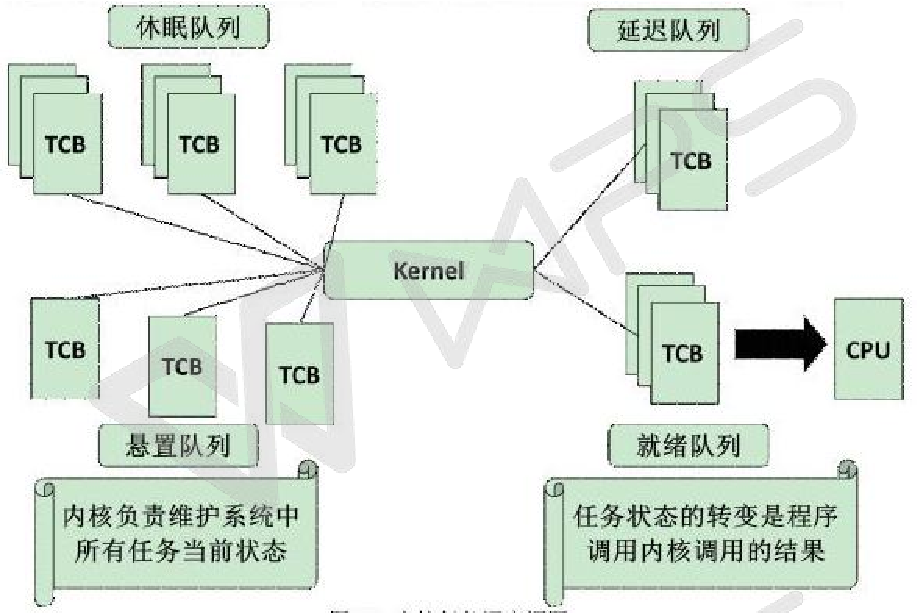
\includegraphics[width=.9\textwidth]{./graphics/vxworks-task-scheduling-diagram.pdf}
\caption{wind任务调度}\label{fig:wind任务调度}
\end{figure}\\
\textbf{任务调度机制:}

	任务调度的基本算法包括:时间片轮转,优先级抢占和独占资源。wind内核这三种算法都有实现,并允许用户自行进行配置。wind将基于优先级的抢占调度作为缺省的调度策略,同级之间的任务依据时间片来进行CPU资源的分配。采用优先级抢占式调度算法符合实时系统的实际需求,紧急情况的出现需要及时的得到响应。这样用户对于需要尽快处理的任务就可以设置一个更高的优先级,保证其时间需求,而相对无关紧要的任务则设置一个较低的优先级。

\subsection{wind任务间通信}
	任务间通信机制可以协调、同步任务之间的活动。在VxWorks中,wind内核提供了三种任务间通信机制(不包括信号机制):信号量,消息队列,管道。这三种机制无一例外的都是在使用共享物理内存机制,只不过这块共享的内存由内核在进行管理,任务无法直接进行访问,而必须通过内核提供的接口函数进行访问,这就提供了一种保护和管理机制,使得任务间通信安全有序的进行。

\begin{enumerate}
	\item \textbf{信号量}
	
	信号量的主要用途是互斥和同步。互斥主要保护资源,即某个时刻只允许只有一个任务在使用该资源。同步则是任务间协同完成某一项共同工作的机制,典型的例子就是生产者和消费者进程,消费者平时处于等待状态,等待生产者完成其资源的生成,而一旦资源产生完毕,此时生产者就会触发同步信号量,让消费者的任务启动(即唤醒)其处理资源的工作。
	
	基于各种资源的不同使用方式,VxWorks信号量机制具体的提供了三种信号量:通用信号量;互斥信号量;资源计数信号量。通用信号量既可用于同步也可用于资源计数,此时资源数通常为 1(当资源数为 1 时,也可以称之为互斥)。互斥信号量针对在使用过程中一些具体问题(如优先级反转)做了优化,更好的服务于任务间互斥需求;资源计数信号量用于资源数较多,同时可供多个任务使用的场合。
	
	VxWorks中信号量是一种指向semaphore结构的指针,其定义如下所示:
\lstset{language=C}
\begin{lstlisting}
typedef struct semaphore
{
  OBJ_CORE objCore;/*对象管理*/
  UINT8 semType; /*信号量类型*/
  UINT8 options; /*信号量选择*/
  UINT16 recurse; /*信号量重复获取计数器*/
  Q_HEAD qHead; /*阻塞的任务队列头*/
  union{
	UNIT count;/*当前状态*/
	struct windTcb *owner;  
  }state;
  EVENTS_RSRC events;/*VxWorks事件*/
}SEMAPHORE;
\end{lstlisting}
	
	\item \textbf{消息队列}
	
	消息队列内核实现上实际是一个结构数组,数组大小和数组中元素的容量在创建消息队列时被确定。消息队列是 Vxworks 内核提供的任务间传递较多信息的一种机制,不过这种机制存在的很大的局限性,即每个消息的最大长度是固定的。Vxworks内核提供的消息机制在创建消息队列时就必须指定单个消息的最大长度以及消息的数量,在消息队列成功创建后,这些参数都是固定不变的。
	
	\item \textbf{管道}
	
	管道相比消息队列提供了一种更为流畅的任务间信息传递机制。消息队列对于每个消息的大
小存在限制,而且必须将信息分批打包,而管道可以像文件那样进行读写,是一种流式消息
机制。管道在底层实现上是一种更为直接的共享物理内存机制。信号量和消息
队列还需要对传递的数据进行某种方式的封装,则管道不会传递信息做任何包装,直接分配
一块连续的内存空间作为任务间信息交互的中转站。传统意义上,管道分为两种:命名管道
和非命名管道。通常任务间通信使用的一般都是命名管道。非命名管道使用在线程意义上,
如父子进程,进程关系密切,且某些变量存在继承关系,如文件描述符,一般无法使用在两
个执行路线完全不同的任务之间。
\end{enumerate}\\		
\textbf{任务间特殊的通信机制--信号:} 信号不是信号量,二者不是一个概念。信号量是一种任务间互斥和同步机制,而信号则用于通知一个任务某个事件的发生。一个信号产生后,对应任务暂停当前执行流程,转而去执行一个特定的函数进行处理。信号机制有些类似于中断,也可以将信号看作是一种用户层提供的软件中断机制(区别于 CPU 本身提供的软件中断指令)。这种用户层软件中断机制相比硬件中断和中断指令而言具有较长的延迟时间,即从信号产生到信号的处理之间大多将经历较长的延迟。Vxworks 下信号处理有些特别,当一个任务接收到一个信号时,在这个任务下一次被调度运行之时进行信号的处理(即调用相关信号处理函数)。事实上,由于 Vxworks 在退出内核函数时都会进行任务调度,故一个任务,无论是否是当前执行任务,都将在被调度运行时执行信号的处理。

	通用操作系统上对于某些信号将不允许用户修改其默认处理函数,如 SIGKILL,SIGSTOP,然而 VxWorks 操作系统中可以对任何信号的处理函数都可以进行更换。

\subsection{I/O系统}
	通常为了实现与应用程序的平台无关性,操作系统都会为应用程序提供一套标准的接口,VxWorks也不例外,这样就可以通过调整底层驱动或者是接近驱动那部分的操作系统中间层来提高应用层开发的效率,避免重复编码。在我们的通用操作系统(如Mac OS、Linux、Windows)当中,通常会将这套应用层的接口标准从操作系统中独立出来,专门以标准库的形式存在,这样可以屏蔽操作系统之间的差异,增强应用程序的平台无关性。
	
	VxWorks中为应用层提供了一套标准的文件操作接口,实际上与GPOS提供接口类似,我们将其称作为标准I/O 库,VxWorks下由ioLib.c文件提供。ioLib.c文件提供如下标准接口函数:creat()、open()、unlink()、remove()、close()、rename()、read()、write()、ioctl()、lseek()、readv()、writev()等\cite{BSP开发人员指南},VxWorks与通用操作系统有很大的一个不同点是:VxWorks不区分用户态和内核态,用户层可以直接对内核函数进行调用,而无需使用陷阱指令之类的机制,以及存在使用权限上的限制。因此VxWorks提供给应用层的接口无需通过外围库的方式,而是直接以内核文件的形式提供。对于一般的设备而言,remove()接口是不需要实现的,\autoref{tab:IO接口函数表} 是七个驱动程序接口函数的简单描述。

\begin{table}[!h]
\centering
\begin{tabular}{|c|c|c|}
\hline
{\hei{接口名称}} & {\hei{函数原型}} & {\hei{描述}}\\ 
\hline
{open} & {open(filename,flags,mode)} & {打开一个新的或已存在的文件}\\
\hline
{create} & {create(filename,flags)} & {创建并打开一个新的文件}\\
\hline
{read} & {read(fd,\& buf,nBytes)} & {从文件中读取}\\
\hline 
{write} & {write(fd,\& buf,nBytes)} & {向文件中写入}\\ 
\hline
{ioctl} & {ioctl(fd,command,arg)} & {其他控制命令}\\
\hline
{close} & {close(fd)} & {关闭文件}\\
\hline
{remove} & {remove(filename)} & {移除文件}\\
\hline
\end{tabular}
\caption{IO接口函数表}\label{tab:IO接口函数表}
\end{table}


\section{USB开发}
	USB(Universial Serial Bus,通用串行总线)是这十几年来应用在PC领域的最新型的接口技术,出现的契机是为了为了解决日益增加的PC外设与有限的主板插槽之间的矛盾,其实现是由一些PC大厂商(Microsoft、Intel等)定制出来的,自从1995年在Comdex上展出以来至今已广泛地被各个PC厂家所支持。目前已经在各类外部设备中都广泛的采用USB接口。USB接口标准目前有三种:USB1.1,USB2.0和USB3.0。USB接口应用如此的广泛是由其独特和实用的特性决定的。

\noindent USB规范规定了USB传输的四种方式,每种方式有各自的用途\cite{USB总线接口开发指南}:
\begin{itemize}
\item \hei{控制传输}\\
	控制传输是每一个设备必须要具有的传输方式,也是四种传输方式中过程最复杂的部分,他使得主机能够从设备列出的范围中读取和选择配置和其他设置,也能够发送自定义请求来为任何目的而发送和接收数据,在配置和列举的过程中起到重要的作用。
\item \hei{批量传输}\\
	批量传输是为了处理传输速率不是很关键的情况,一般用于打印机和扫描仪。
\item \hei{中断传输}\\
	中断传输是为了那些要快速实现主机和设备的交互而准备的,比如适用于鼠标和键盘。
\item \hei{等时传输}\\
	等时传输用于必须要按照一个常数传输数据的情况,比如一个需要被实时播放的视频/音频数据流。
\end{itemize}\\
所有的传输都是由事务组成,事务又由包组成,而包包含一个包识别器(PID)、CRC和其他的信息\cite{USB大全}。

	USB的体系结构如\autoref{fig:USB体系结构}所示
\begin{figure}[!h]
\centering
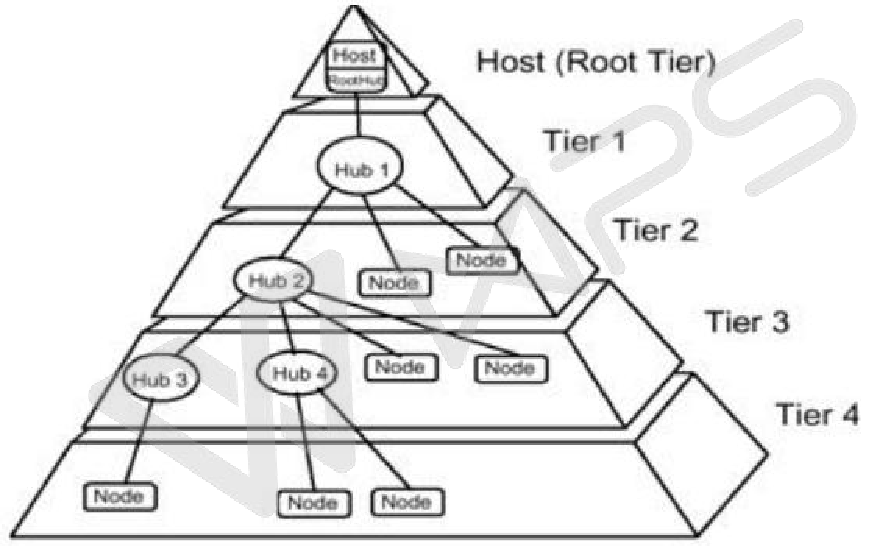
\includegraphics[width=1.0\textwidth]{./graphics/usb-structure.pdf}
\caption{USB总线拓扑结构}\label{fig:USB体系结构}
\end{figure}

	USB的物理层拓扑为星型结构,包括三个部分:USB主机(Host)、USB集线器(Hub)、USB设备(Device)。
	
\begin{enumerate}
\item \textbf{USB主机}

	USB的体系结构只允许系统中有一个主机,主计算机系统的USB接口称之为USB主控制器。主控制器可以是硬件、固件或软件的联合体,其控制着总线上所有USB设备和所有集线器的数据通信过程。所有的数据传输都是由USB的主机端发起的,而且如果USB主机嵌入在一个计算机系统中,在数据的传输过程中也不需要计算机的CPU参与传输工作。USB主机通常具有以下的功能:
	\begin{itemize}
	\item 检测USB设备的插拔动作(通过根集线器来实现)
	\item 管理 USB 主机和USB设备之间的控制流
	\item 管理USB主机和USB设备之间的数据流
	\item 收集USB主机的状态和USB设备的动作信息
	\end{itemize}
\item \textbf{USB集线器}
	
	根集线器是集成在主机系统当中的一个特殊集线器,他可以提供一个或者跟多的接入口。在即插即用的USB体系结构当中,集线器是一种很重要的设备。其极大的简化了USB的复杂性,而且以很低的价格和易用性提供了设备的健壮性,一个集线器通常会包括两个部分:集线控制器和集线放大器。集线放大器是一种在上游端口v和下游端口之间的协议控制开关。集线控制器提供接口寄存器用于和主机之间的通信,允许主机对其特定状态和控制命令进行设置,并监视和控制其端口。

每个集线器的下游端口都可以连接另外的集线器或功能部件,最大的连接能力是127,集线器可以检测每一个下游端口的设备的安装或移除,并可以对下游端口的设备分配资源,每一个下有端口都有独立的能力,不论是高速或者是低俗设备均可连接。集线器可以将低俗和高速端口的信号分开。

\item \textbf{USB设备}

	USB设备是USB总线系统的重要组成部分,它们以从属的方式与USB主机进行通信,并受USB主机的控制。USB主机端提供的协议软件通过和USB设备通信获得设备的信息,并给设备提供驱动程序,相比USB主机而言,USB设备只能够被动的应答,按照USB主机的要求接受或者发送数据。USB设备通过以下的属性来完成主机的要求:
	\begin{itemize}
	\item \textbf{描述符}\\
	USB协议为USB设备定义了一套描述设备功能和属性的固定结构的描述符,通过这些描述符向USB主机汇报设备的各种属性,主机通过对这些描述符的访问对设备进行识别、配置并为其提供相应的客户端驱动程序。典型的描述符一般由USB标准描述符和USB类描述符,或者由USB标准描述符和USB厂商特定描述符组成。运行于USB协议栈上层的客户端驱动程序通过这些信息正确的访问设备并与其进行通信,以实现即插即用的目的。
	\item \textbf{类}\\
	USB协议支持许多的外围设备,为了正确的驱动这些设备,USB主机端要为这些设备提供符合USB协议的驱动程序,称为客户端驱动。同时为了避免客户端程序过多,协议通过归纳将设备划分为不同的设备类,把功能相近的设备归为一类,主机端只需要提供类驱动程序便可以驱动大多数的USB设备。	
	\item \textbf{功能(Function)/接口(Interface)}\\
	在USB协议中,Function被定义为具有某种能力的设备,即相当于传统的单一功能设备。随着USB设备应用的发展,物理上几种不同的Function可以组成一台设备,只要设备的接口具有某种独立的能力,就称为一个Function。Function是从功能角度来说的,从设备的角度来说,它又被称为Interface。
	\item \textbf{端点(Endpoint)}\\
	端点层的各个子模块是USB设备与USB主机逻辑上的数据传输的最基本单元,即最基本的通信点,因而端点层的每一个逻辑模块被称为端点(Endpoint)。每一个端点都关联一个相应的端点号和数据传输方向(IN/OUT)。具有相同端点号和不同传输方向的通信点表示不同的端点,端点0被USB规范保留用作设备枚举和配置过程中的数据传输端点,与端点0对应的管道是默认管道,设备的所有端点共享端点0。在一个USB系统当中,USB主机对特定设备功能的访问是通过使用不同的端点号,否则,USB主机将不能对相应的设备进行正确的访问。由于在系统运行时,不同的设备配置有着互斥性,因而在不同的配置描述中,端点号是可以重复的。
	\item \textbf{管道}\\
	设备端点与USB主机所形成的具有特定数据传输特性(如数据传输格式、传输带宽、传输方向等)的数据通道,被称为管道。管道的物理介质就是USB系统中的数据线。端点层的USB设备与USB主机之间的数据传输都是基于管道进行的。
	\item \textbf{设备地址}\\
	USB主机的客户端驱动程序通过描述符来区分不同的设备,而USB主机控制器通过设备地址来区分设备。设备地址共有7位,表示理论上系统可以同时连接127个USB设备,但是在实际中,由于USB总线带宽的限制,这么多设备不可能同时的工作。USB主机负责为USB系统中的设备分配不同的设备地址,用来表示哪个设备的同时还要指名设备的端点号,表示使用哪个管道。
	\end{itemize}	
	
\end{enumerate}

	一个主机和设备的连接需要一些列的层次和实体之间的交互,USB接口层在主机和设备间提供物理、信号包的关联,USB设备层表示USB系统程序实现对一个设备进行的总的USB操作,功能层适当匹配的客户服务程序层提供附加的功能给主机。设备和功能层当中各自有逻辑通信,但是实际的USB数据传输是通过USB总线接口层来实现的\cite{USB开发手册}\cite{圈圈教你玩USB}。


\section{CP2102开发}

	计算机与计算机或计算机与终端设备之间的通信方式有串口通信,并行通信以及网络通信等。串口是单个设备实现计算机接入常使用的一种方式,串口的硬件实现简单,在以前的设备中广泛使用。使用串口通信方式的优点是成本低,使用线路少,由于串口的数据和控制信息是一位接一位的串行地传输下去的,比较适合于远距离传输。但是串口也有传输速度慢,扩展不方便等问题,因此其发展受到限制,导致其渐渐在设备上消失。而USB接口因速度快、连接灵活、支持即插即用等特点成为了设备标配接口,RS232和USB虽然都是属于串行接口, 但是他们的数据格式、通信协议以及信号电平定义和机械连接方式都完全不同\cite{何源2006USB}。
	
	在平常的生产实践和科学研究当中经常需要在上位机和下位机中进行数据和控制的传输,这种数据、控制传输都需要通过串口来进行,于是需要通过一些手段将USB转换为串口,这时就出现了一些专用的USB转UART芯片,CP2102就是这样一种芯片。CP2102与其他同类型的芯片相比具有功耗更低、体积更小、集成度更高(仅需少量外部元件)、价格更低等优点。因此我们此次选择这个芯片作为调通道的设计当中使用的芯片。	

\subsection{RS232与TTL}
	我们通常见到的串口有两种的物理标准,D型9针(对应于RS-232标准)插头和4针(对应于TTL标准)的杜邦头,4针的通常也会有第五根引脚--3.3V电源引脚。RS232电平标准用正负电压来表示逻辑状态,在RS-232标准中正电压是0,负电压是1。TTL电平标准使用高低电平来表示逻辑状态,TTL标准中低电平是0,高电平是1。使用TTL标准进行连接时,一般只会使用GND、RXD、TXD引脚,不会使用VCC或3.3V的电源线,避免与目标设备上的供电冲突。
	PL2303、CP2102芯片是USB转TTL串口的芯片,用USB来扩展串口(TTL)电平。
	
 
\subsection{CP2102特性}
	CP2102是SILICON LABORATORIES推出的USB与RS232接口转换芯片,是一种高度集成的USB-UART桥接器,提供一个使用最小化的元件和PCB空间实现RS232转USB的简便的解决方案。
	CP2102芯片包含有一个USB2.0全速功能控制器,EEPROM,USB收发器,振荡器和带有全部的调制解调器控制信号的异步串行数据总线(UART),CP2102将全部的部件集成在一个5mm*5mm MLP-28封装的IC当中\cite{CP2102},cp2102的电路框图如\autoref{fig:cp2102电路框图}所示。

\begin{figure}[!h]
\centering
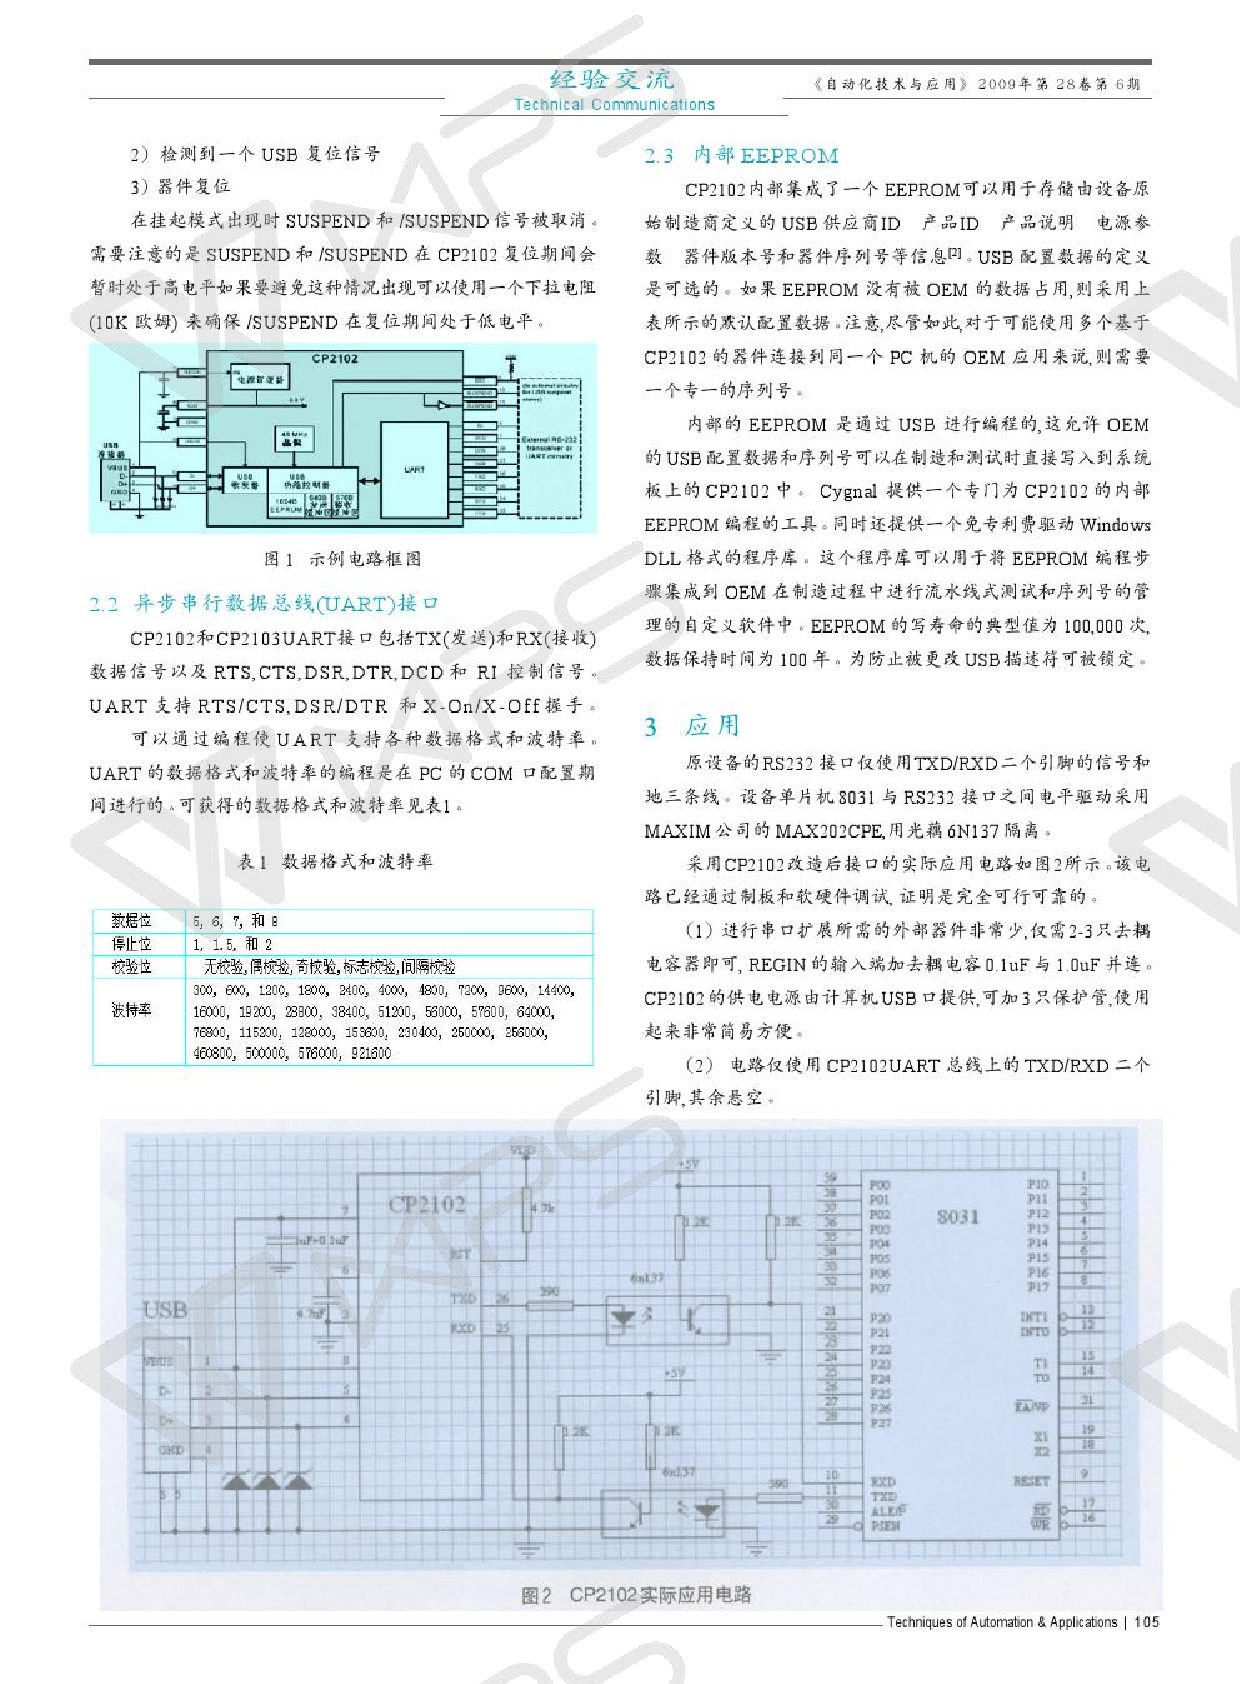
\includegraphics[width=1.0\textwidth]{./graphics/cp2102-circuit-diagram.pdf}
\caption{cp2102电路框图}\label{fig:cp2102电路框图}
\end{figure}

	CP2102可以完成USB/RS-232双向转换(需要外接一个TTL电平到RS-232电平的芯片),一方面可以从主机接收USB数据并将其转换为RS232信息格式流发送给外设,另外一方面可以从RS232外设接收数据转换为USB数据格式传送回主机,这些工作都会由芯片自动完成\cite{何源2006USB}。使用时我们只需要将数据通过USB的数据包发送给CP2102芯片即可,芯片会自动进行解析和控制。在我们本次的使用当中只需要将其转换为TTL标准即可完成需求,不需要转换成RS-232电平,因此CP2102模块之外不再需要额外的转换为RS-232电平的芯片。
		
\begin{enumerate}
\item CP2102的USB功能控制器和收发器:CP2102的USB功能控制器是一个符合USB2.0协议的全速器件,这个器件负责管理USB和UART之间的所有数据传输以及由USB主控制器发出的命令请求和用于控制UART功能的命令。
\item 异步串行数据总线(UART)接口:CP2102的UART接口包括TXD(发送)和RXD(接收)数据信号以及RTS,CTS,DSR,DTR,DCD和RI控制信号。ART支持RTS/CTS,DSR/DTR和X-on/X-Off握手。且支持编程使UART支持各种数据格式和波特率。ART的数据格式和波特率的编程是在PC的COM口配置期间进行的。可以使用的数据格式和波特率见\autoref{CP2102可配置参数}。
\item 内部EEPROM:CP2102内部集成了一个EEPROM用于存储设备原始制造商定义的USB供应商ID、产品ID、产品说明、电源参数、器件版本号和器件序列号等信息\cite{CP2102}。USB配置数据的定义是可选的,如果EEPROM没有被OEM的数据所填充的话,则设备会自动的使用一组默认的数据如\autoref{CP2102DefaultConfigure}所示。
\end{enumerate}

\begin{table}[!h]
\centering
\begin{tabular}{|c|c|}
\hline
{数据位} & {5,6,7,8} \\
\hline
{停止位} & {1,1.5,2} \\
\hline
{校验位} & {无校验,偶校验,奇校验,标志校验,间隔校验} \\
\hline
{波特率} & \tabincell{c}{600,1200,2400,4800,7200,9600,14400,16000,19200,28800,\\ 38400,51200,56000,57600,64000,76800,115200,128000,158600,\\ 230400,250000,256000,4608000,576000,921600}\\
\hline
\end{tabular} 
\caption{CP2102可配置参数}\label{CP2102可配置参数}
\end{table}

\begin{table}[!h]
\centering
\begin{tabular}{|c|c|}
\hline
{\hei{Name}} & {\hei{Value}} \\
\hline
{Vendor ID} & {10C4h} \\
\hline
{Product ID} & {EA60h} \\
\hline
{Power Descriptor(attributes)} & \tabincell{c}{80h}\\
\hline 
{Power Descriptor(Max Power)} & {32h} \\
\hline
{Release Number} & {0100h} \\
\hline
{Serial Number} & {0001(63 characters maximum)} \\
\hline
{Product Description String} & \tabincell{c}{"CP2102 USB to UART Bridge Controller”(126 characters maximum)"} \\
\hline
\end{tabular}
\caption{CP2102默认配置表}\label{CP2102DefaultConfigure}
\end{table}


\subsection{CP2102应用}
	使用CP2102开发USB口转串口具有电路简单,运行可靠,成本低廉的优点,通常在使用CP2102进行串口扩展的时候所需要的外部器件是非常少的,仅仅需要2-3个去耦电容即可,在silicon给出的文档当中已经帮我们给出了一个最简单的连接电路图,如\autoref{fig:cp2102电路框图}所示,由于我们并不需要将TTL电平转换为RS-232电平,所以我们不需要额外的电平转换芯片。电路使用CP2102UART总线上的TXD/RXD两个引脚,其余的引脚都悬空。此次我们使用的是购买的已经制作好的CP2102转TTL模块,如\autoref{fig:cp2102模块正反面}所示:
\begin{figure}[h]
\centering
  \begin{subfigure}[b]{0.4\textwidth}
  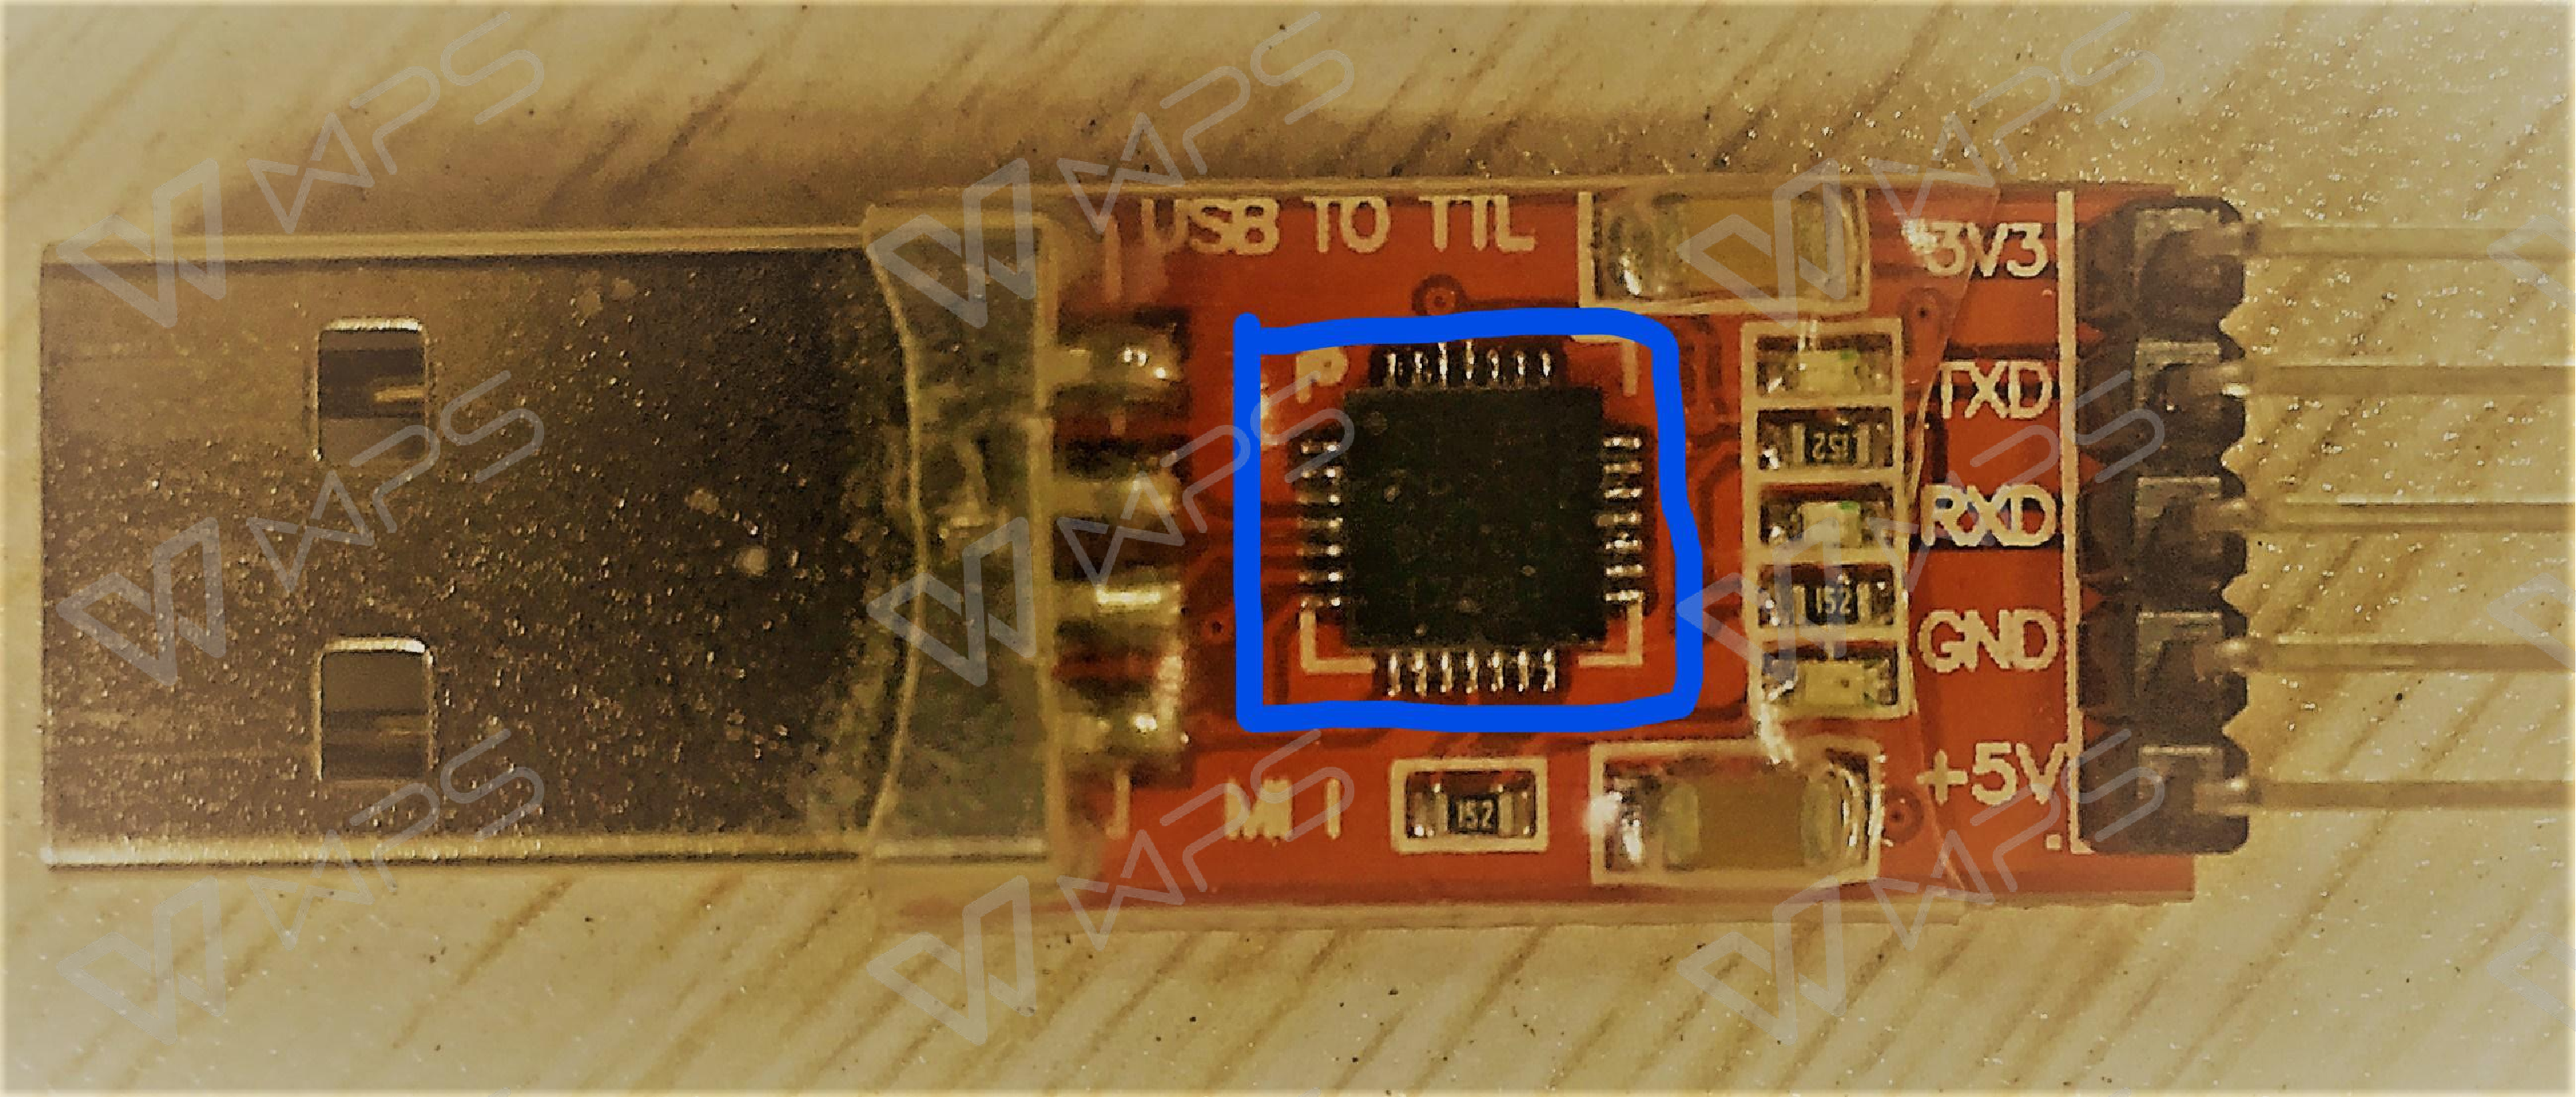
\includegraphics[width=\textwidth]{./graphics/cp2102Front.pdf}
  \caption{CP2102模块正面}\label{fig:cp2102Front}
  \end{subfigure}
  ~
  \begin{subfigure}[b]{0.4\textwidth}
  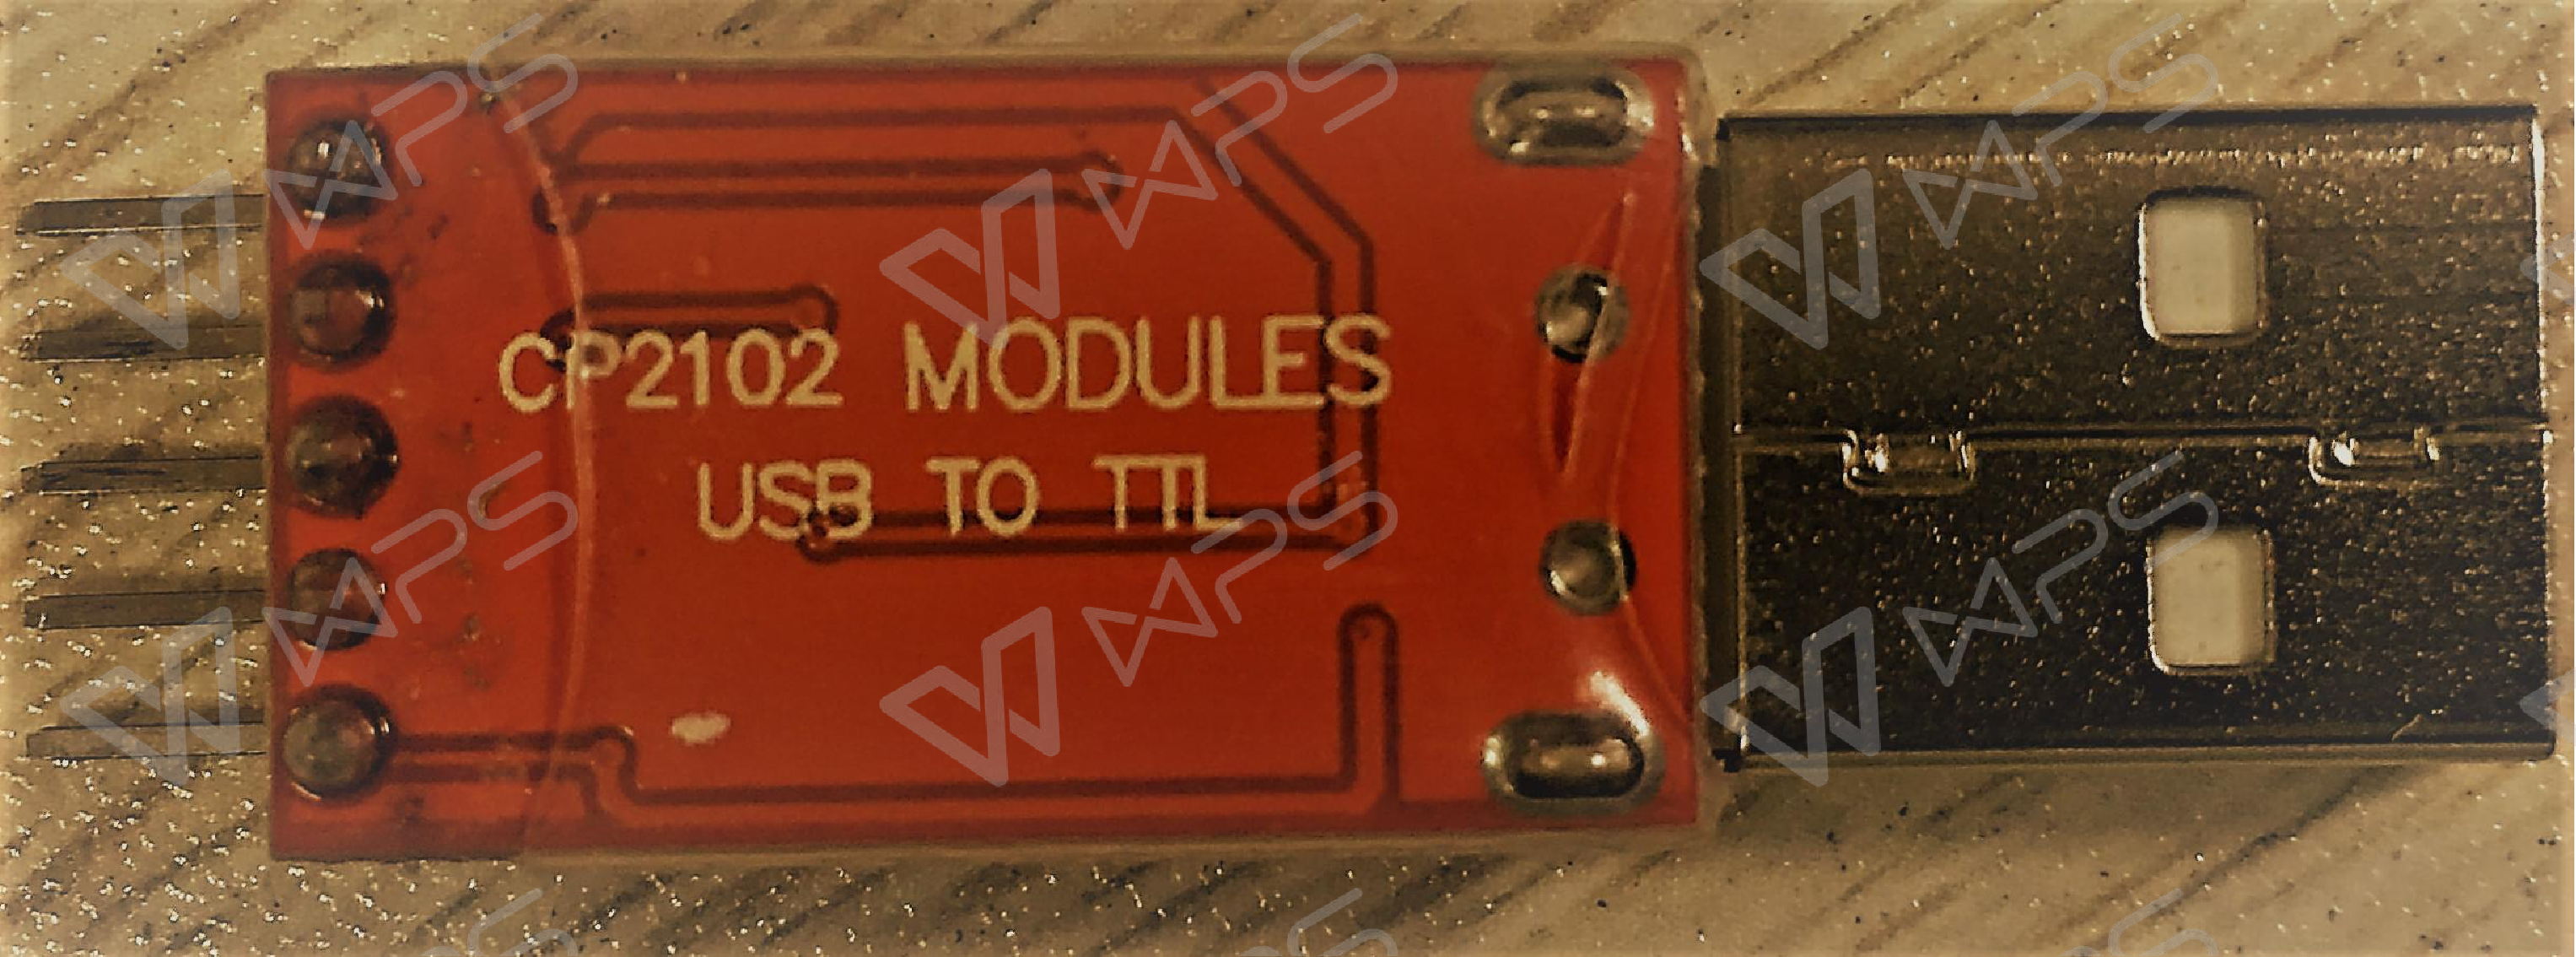
\includegraphics[width=\textwidth]{./graphics/cp2102Rear.pdf}
  \caption{CP2102模块反面}\label{fig:cp2102Rear}
  \end{subfigure}
\caption{CP2102模块正反面}\label{fig:cp2102模块正反面}
\end{figure}

CP2102当中的协议控制单元会通过接受USB接口的命令,对UART接口进行配置(如配置通信的波特率、数据位、校验位、起始/停止位、流控信号等)。CP2102当中的接收和发送缓冲区用来临时保存双方在数据传输过程中的数据。以从计算机到外设的数据传输为例。当USB转串口设备连接到PC的USB总线上时,PC在检测到设备连接之后会对设备进行初始化并启动相关的客户端驱动程序;之后会由驱动程序给设备发送配置命令,设置设备的数据传输特性;最后,在数据传输的时候,计算机上的驱动程序会将数据包传输给USB接口(通常使用批量传输的方式),设备从USB接口提取出数据并保存在数据缓冲区中,UART接口再从数据缓冲区中将数据取走并发送出去,从外设传输数据到计算机的方式则相反。

\section{软件需求}

	整个调试通道的设计包括两个部分,一个是应用层的接口的设计,一个USB口转串口的驱动程序的设计。整个系统的结构如\autoref{fig:debug-system-diagram}所示:
\begin{figure}[!h]
\centering
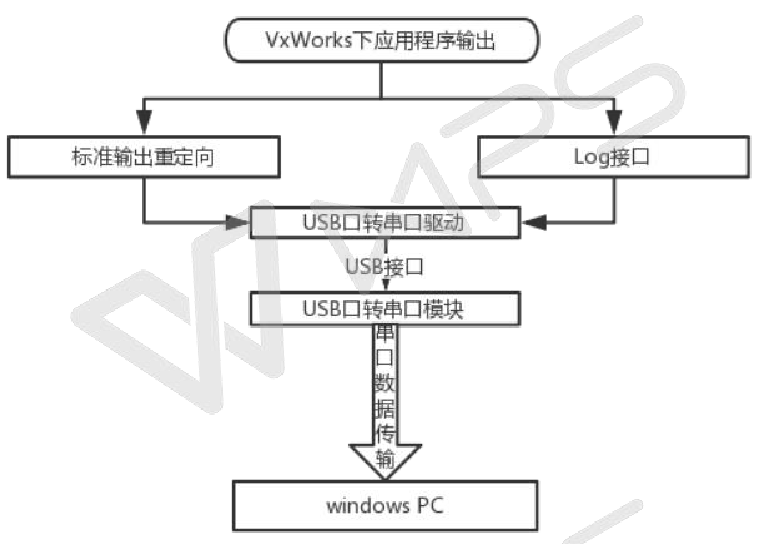
\includegraphics[width=.7\textwidth]{./graphics/debug-system-diagram.pdf}
\caption{调试通道整体结构图}\label{fig:debug-system-diagram}
\end{figure}

应用层的接口包括两个部分:一是标准输出重定向接口的设计,目的是在程序运行期间直接调用标准输出函数时就能够将输出信息通过我们的串口输出出去,但是这个标准输出输出的信息不是格式化的信息。二是Log接口函数,通过调用这个接口函数可以将调试信息格式化输出,输出信息会自动包括调试的级别、产生的时间、所处的文件、行号等信息,便于对调试信息进行分析。

主要的模块包块一下几个:
\begin{itemize}
\item \hei{ResetStdOut():} 提供给用户选择是否需要重定向标准输出,若参数为1则将标准输出进行重定向,若参数为0,则关闭标准输出重定向,恢复到之前的标准输出。

\item \hei{Log接口函数:} 提供封装的不同级别的Log调试接口,包括LogE(表示错误信息)、LogD(表示详情信息)、LogW(表示警告信息)、LogI(表示)
\end{itemize}

	
	作为非标准类型的USB设备,CP2102 USB-TTL模块连接到主机之后必须使用一个由开发者自己编写的设备驱动程序来驱动其正常工作,而PC端的应用程序则无需任何更改,仍将其当做一个正常的串口设备来使用即可,但是本质上所有针对该串口发起的通信都是通过USB总线来传输的。而对于设备一方,收发的都是TLL的电平的串行数据。利用现有的CP2102模块能够轻松地完成USB-TTL的转换,开发者无需考虑总线枚举、数据收发与转换等工作,这些都由芯片自动完成。
	
	在windows和Linux下都有已经实现好了的基于CP2102的USB口转串口的驱动,但是在VxWorks下并没有这个驱动的实现,我们的调试通道的核心部分正是这个USB口转串口的驱动,因此我们需要在VxWorks中自己实现这个驱动程序。
		



